
\chapter{Introduction}
 
 {\slshape \scshape ``You have to be in a state of play to design. If you're not in a state of play, you can't build anything." - Paula Scher}

Mechatronics is an amalgam of mechanical electronics: systems that contain both mechanical and electrical components. It's a field that spans nearly every industry, so any one source (even this one) will not be complete with all the information you need. But this may be a good jumping off point. I'm writing this generally towards those in a competitive robotics environment, so will use many examples from there, but you soon find that those same technologies that shoot foam balls into goals can be used anywhere from assembly lines to emergency medical equipment.

This document is not intended to be all-encompassing. In reality, it's just an outline; a map. We live in an era where information is readily available on net demand. This document really doesn't contain anything new. Its goal is to show you a plethora of things that exist in a breadth-first fashion before you dive down a particular rabbit hole. There are a few places where I'll dive deeper because I feel it's relevant to show you some of the nuances you should be aware of. By and large, my goal isn't to drill home every single thing because I'll fail at that and fail you in the process. Someone will come up with something new, or improve something discussed here, and this information will become outdated. I'll try to keep it up to date... but I will definitely fail!

The human mind is a weird thing. It's better at prompted recall than unprompted recall. You may not always be thinking about the many different types of bolts, but if you've seen that before, and you come across a problem that needs that information, you'll find you might be able to figure it out - or at least know where to start looking.

I hope to keep this terse. We're going to go fast and I'm going to leave some things to your imagination or research to figure out exactly how they work. I love mechatronics and hope you do too, so I don't want to spoil it by chewing your steak for you. With that... let's begin.

\chapter{Terminology}

\section{Stresses and Deformations}
\begin{figure}[H]
\begin{subfigure}[b]{.32\linewidth}
	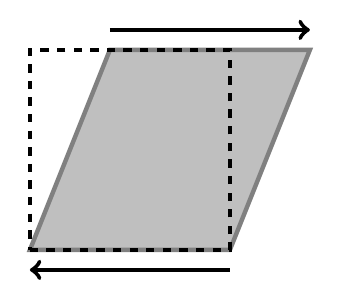
\begin{tikzpicture}[x=1.0in, y=1.0in]
	  %\fill[lightgray] (1.0,0)--(0,1.0)--(0,0)--cycle;
	  \filldraw[color=gray, fill=lightgray, ultra thick] (0,0) -- (1,0) -- (1.4,1) -- (0.4,1) -- cycle;
	  \draw[black, ultra thick, dashed] (0,0) -- (1,0) -- (1.0,1) -- (0.0,1) -- cycle;
	  \draw[black, ->, ultra thick] (1,-0.1) -- (0,-0.1);
	  \draw[black, ->, ultra thick] (0.4,1.1) -- (1.4,1.1);
	\end{tikzpicture}
	\caption{Shear}
\end{subfigure}\begin{subfigure}[b]{.32\linewidth}
	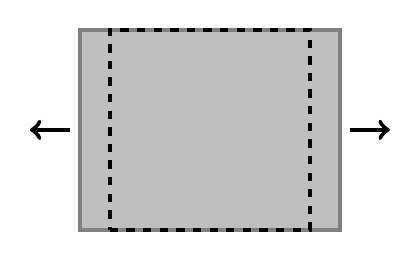
\begin{tikzpicture}[x=1.0in, y=1.0in]
	  %\fill[lightgray] (1.0,0)--(0,1.0)--(0,0)--cycle;
	  \filldraw[color=gray, fill=lightgray, ultra thick] (-0.15,0) -- (1.15,0) -- (1.15,1) -- (-0.15,1) -- cycle;
	  \draw[black, ultra thick, dashed] (0,0) -- (1,0) -- (1.0,1) -- (0.0,1) -- cycle;
	  \draw[black, ->, ultra thick] (-0.2,0.5) -- (-0.4,0.5);
	  \draw[black, ->, ultra thick] (1.2,0.5) -- (1.4,0.5);
	  \draw[black, ->, ultra thick, opacity=0] (1,-0.1) -- (0,-0.1);
	\end{tikzpicture}
	\caption{Axial / Tension}
\end{subfigure}\begin{subfigure}[b]{.32\linewidth}
	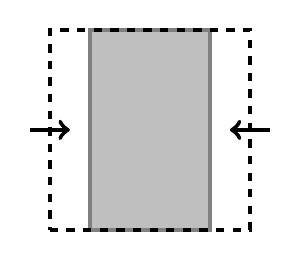
\begin{tikzpicture}[x=1.0in, y=1.0in]
	  %\fill[lightgray] (1.0,0)--(0,1.0)--(0,0)--cycle;
	  \filldraw[color=gray, fill=lightgray, ultra thick] (0.2,0) -- (0.8,0) -- (0.8,1) -- (0.2,1) -- cycle;
	  \draw[black, ultra thick, dashed] (0,0) -- (1,0) -- (1.0,1) -- (0.0,1) -- cycle;
	  \draw[black, <-, ultra thick] (0.1,0.5) -- (-0.1,0.5);
	  \draw[black, <-, ultra thick] (0.9,0.5) -- (1.1,0.5);
	  \draw[black, ->, ultra thick, opacity=0] (1,-0.1) -- (0,-0.1);
	\end{tikzpicture}
	\caption{Axial / Compression}
\end{subfigure}

\begin{subfigure}[b]{.47\linewidth}
	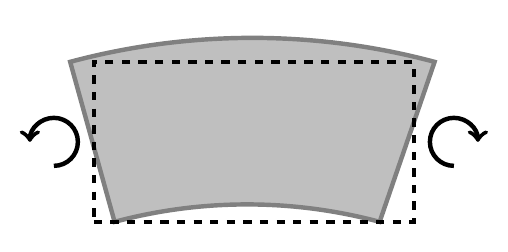
\begin{tikzpicture}[x=0.8in, y=0.8in]
	  %\fill[lightgray] (1.0,0)--(0,1.0)--(0,0)--cycle;
	  \filldraw[color=gray, fill=lightgray, ultra thick] ({0.5*sin(15)},-0.5) arc(105:75:3.2) -- ({2+0.5*sin(15)},0.5) arc(75:105:4.4) -- cycle;
	  \draw[black, ultra thick, dashed] (0,-0.5) -- (2,-0.5) -- (2,0.5) -- (0,0.5) -- cycle;
	  \draw[black, <-, ultra thick] (-0.4,0) arc(180:-90:0.15);
	  \draw[black, <-, ultra thick] (2.4,0) arc(0:270:0.15);
	\end{tikzpicture}
	\caption{Bending}
\end{subfigure}\begin{subfigure}[b]{.47\linewidth}
	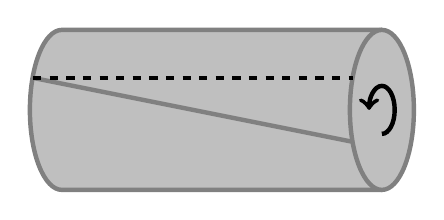
\begin{tikzpicture}[x=0.8in, y=0.8in]
	  \filldraw[color=gray, fill=lightgray, ultra thick] (2,-0.5) -- (0,-0.5) arc (270:90:0.2 and 0.5) -- (2,0.5);
	  \filldraw[color=gray, fill=lightgray, ultra thick] (2,0) circle[x radius=0.2, y radius=0.5];
	  \draw[color=gray, ultra thick] (-0.18, 0.2) -- (1.82, -0.2);
	  \draw[color=black, ultra thick, dashed] (-0.18, 0.2) -- (1.82, 0.2);
	  %\draw[black, <-, ultra thick] (-0.3,0) arc(0:270:0.08 and 0.15);
	  \draw[black, <-, ultra thick] (1.92,0) arc(180:-90:0.08 and 0.15);
	\end{tikzpicture}
	\caption{Torsion}
\end{subfigure}

\begin{subfigure}[b]{.95\linewidth}
	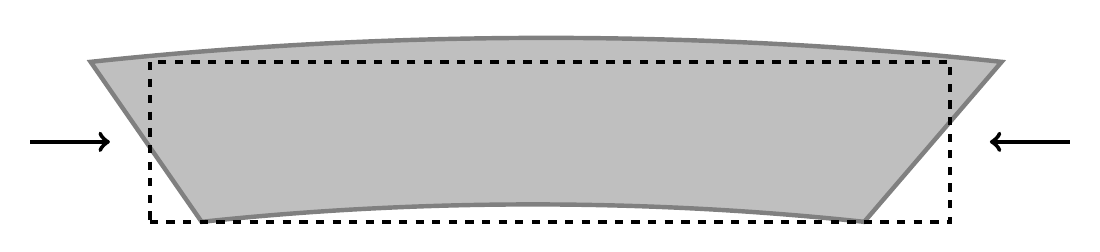
\begin{tikzpicture}[x=2.0in, y=0.8in]
	  %\fill[lightgray] (1.0,0)--(0,1.0)--(0,0)--cycle;
	  \filldraw[color=gray, fill=lightgray, ultra thick] ({0.5*sin(15)},-0.5) arc(105:75:3.2) -- ({2+0.5*sin(15)},0.5) arc(75:105:4.4) -- cycle;
	  \draw[black, ultra thick, dashed] (0,-0.5) -- (2,-0.5) -- (2,0.5) -- (0,0.5) -- cycle;
	  \draw[black, <-, ultra thick] (-0.1,0) -- (-0.3,0);
	  \draw[black, <-, ultra thick] (2.1,0) -- (2.3,0);
	\end{tikzpicture}
	\caption{Buckling}
\end{subfigure}

\end{figure}

\section{Directions on Rotating Components}
\begin{figure}[H]
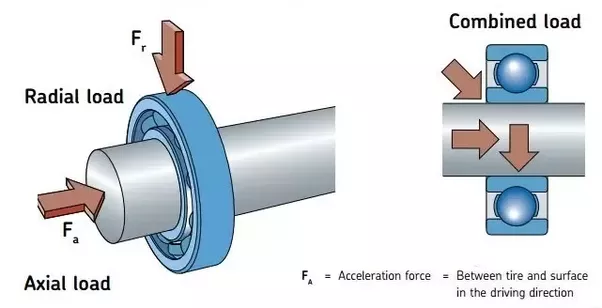
\includegraphics[width=0.8\textwidth]{imgs/radial_axial.png}
\caption{Axial vs. radial directions.}
\end{figure}
%TODO: Tangential, angular